\section{Simulation Analysis}
\label{sec:simulation analysis}
\subsection{t$<$0}


The following tables show the simulated and theoretical operating point results for the study case circuit, for t$<$0.

Note that aldr is not a real node, but it is needed for ngspice calculations.

\vspace{0.5cm}
\begin{table}[!htb]
    \begin{minipage}{0.50\textwidth}~
        \centering
        \begin{tabular}{|l|r|}
        {\bf Name} & {\bf Value [V]} \\ \hline
        \input{../sim/circ1_tab}
      \end{tabular}
      \caption{Simulation Results}
     \end{minipage}%
     \begin{minipage}{0.50\textwidth}~
       \centering
       \csvautotabular{resultados1.txt}
       \vspace{0.62cm}
       \caption{Theoretical results.}
     \end{minipage}
     \label{tab:t0}
\end{table}

%\vspace{0.5cm}
% Section 3.2 *******************************
\subsection{t $=$ 0}
\label{sec:3.2}
%\vspace{0.5cm}

The following tables show the simulated and theoretical operating point results for the study case circuit, for t$=$0. Note that aldr is not a real node, but it is needed for ngspice calculations.

%\vspace{0.5cm}

\begin{table}[!htb]
    \begin{minipage}{0.50\textwidth}~
        \centering
        \begin{tabular}{|l|r|}
        {\bf Name} & {\bf Value [V]} \\ \hline
        \input{../sim/circ2_tab}
      \end{tabular}
      \caption{Simulation Results}
     \end{minipage}%
     \begin{minipage}{0.50\textwidth}~
       \centering
       \csvautotabular{resultados2.txt}
       \vspace{0.62cm}
       \caption{Theoretical results.}
     \end{minipage}
     \label{tab:t0}
\end{table}


To simulate the operating point for $V_s(0)$, the capacitor was replaced with a voltage source $V_x$ = V(6)-V(8), where V(6) and V(8) are the voltages in nodes 6 and 8 obtained in 3.1.. This step is needed because the capacitor will discharge through the resistor but this takes time, therefore: $V_c=V_c(t<0)=V(6)-V(8)$. This is necessary to calculate the "base" voltage in the specified nodes, to be used as a boundary condition in the following analyses. Note that even though the results may seem different, they are quite similar. Note that the powers in the simulation results are quite low, so they are approximately zero.

\vspace{0.5cm}
% Section 3.3 ***********************
\subsection{Natural response using \ref{sec:3.2}'s boundary conditions }

The Table~\ref{fig:trans3} shows the simulated natural solution results for the study case circuit. It is possible to denote that the results are similar. Both cases show V(6).

\begin{figure}[!htb]
    \minipage{0.45\textwidth}
      \includegraphics[width=\linewidth]{../sim/trans3.pdf}
      \caption{Natural response from ngspice}
      \label{fig:trans3}
    \endminipage\hfill
    \minipage{0.45\textwidth}
      \includegraphics[width=\linewidth]{circ2.png} %../sim/
      \caption{Natural response from matlab}
      
    \endminipage\hfill
\end{figure}




%\vspace{1.0cm}
% Section 3.4 ***********************
\subsection{Natural and forced response using \ref{sec:3.2}'s boundary conditions }

Figure~\ref{fig:trans4} shows the simulated  Natural and forced response results for the study case circuit, calculated from ngspice.

\begin{figure}[!htb] \centering
    \minipage{0.45\textwidth}
      \includegraphics[width=0.8\columnwidth]{../sim/trans4.pdf}
      \caption{Stimulus and Response from Ngspice}
      \label{fig:trans4}
    \endminipage\hfill
    \minipage{0.45\textwidth}
      \includegraphics[width=\linewidth]{tot_ponto5.png} %../sim/
      \caption{Stimulus and Response from Matlab}
    \endminipage\hfill
\end{figure}



%\vspace{50.0cm}
% Section 3.5 ***********************
\subsection{Frequency response using \ref{sec:3.2}'s boundary conditions }
As explained in \ref{sec:2.4}, the changes in the frequency and phase responses are characteristic of a low passing filters.

\begin{figure}[!htb]
    \minipage{0.45\textwidth}
      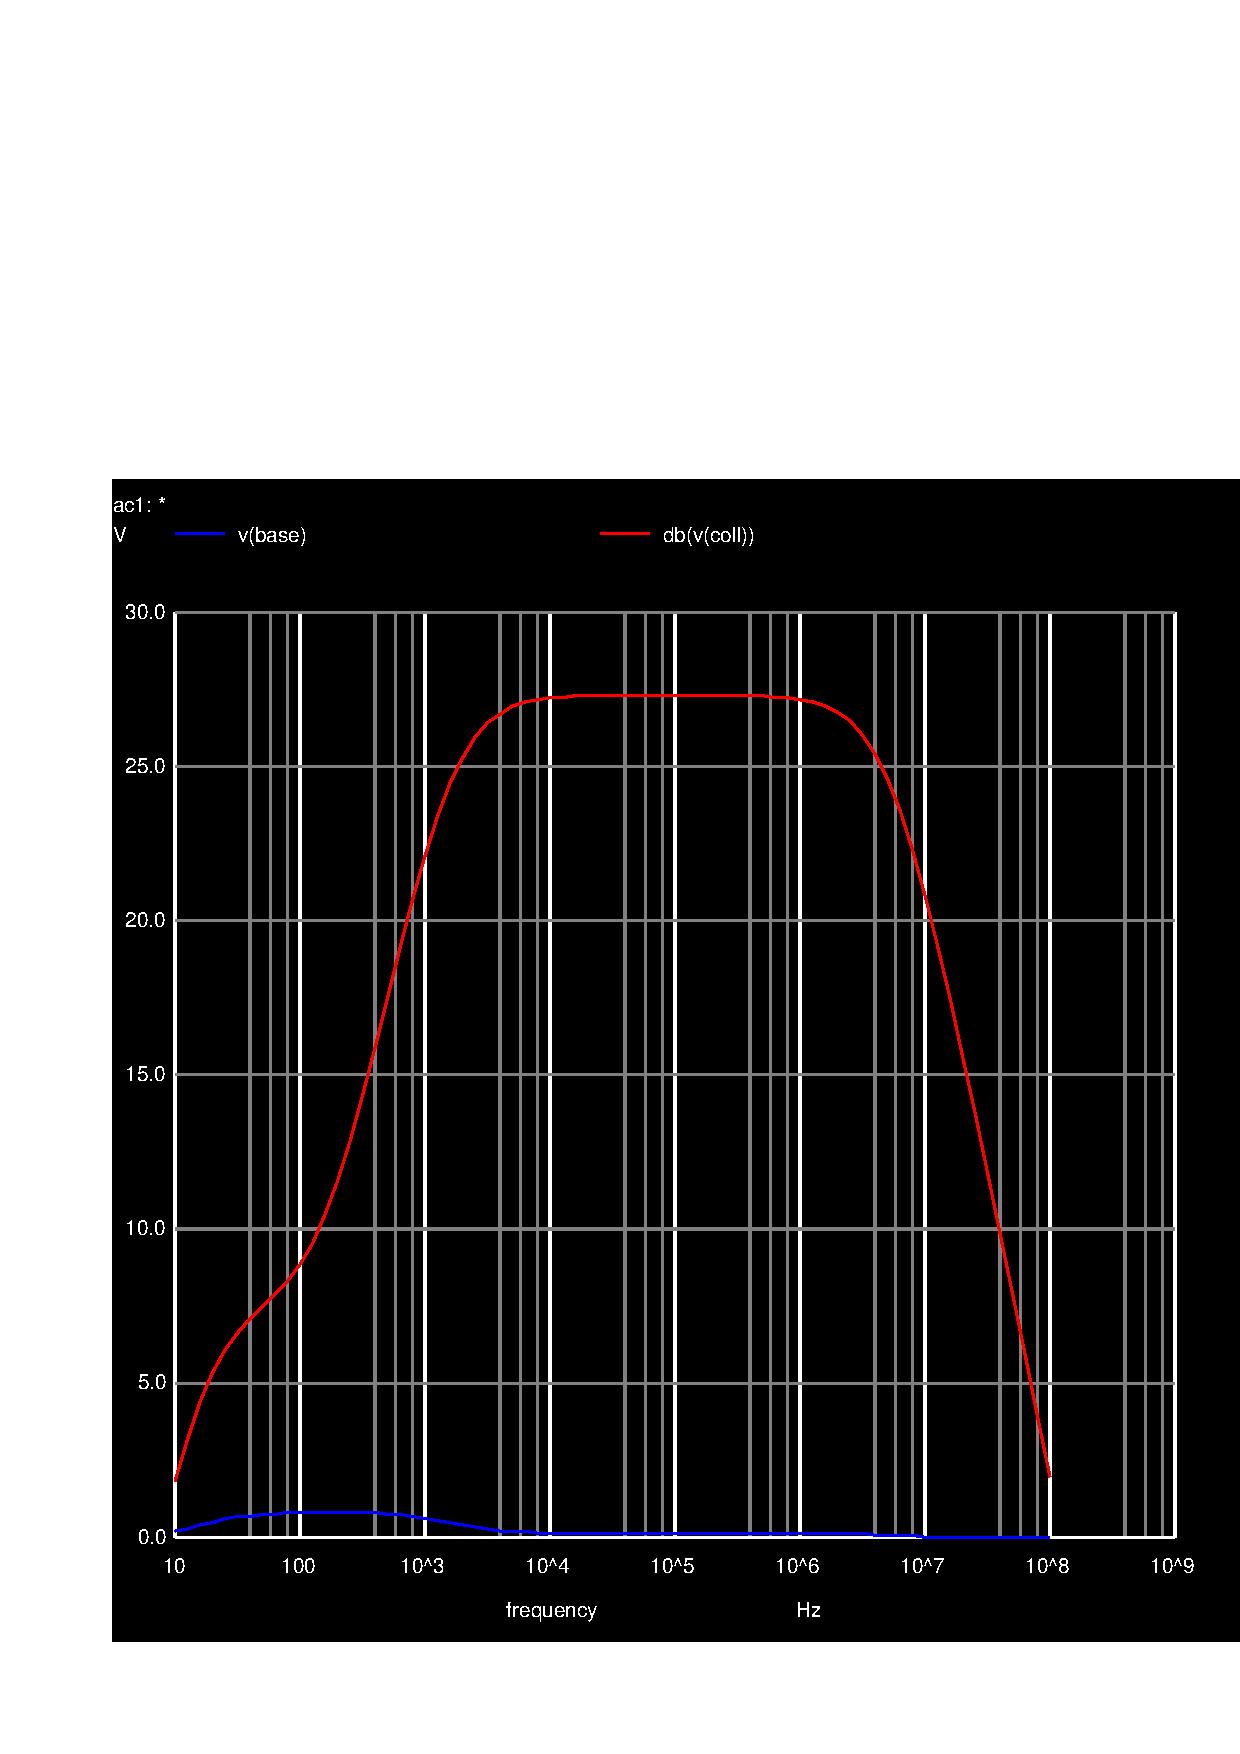
\includegraphics[width=0.8\columnwidth]{../sim/acm.pdf}
      \caption{Frequency response from ngspice}
      \label{fig:trans5}
    \endminipage\hfill
    \minipage{0.45\textwidth}
      \includegraphics[width=\linewidth]{T_abs_zoom.png} %../sim/
      \caption{Frequency response from matlab}
    \endminipage\hfill
\end{figure}



\vspace{2.0cm}


\begin{figure}[h]
    \minipage{0.45\textwidth}
      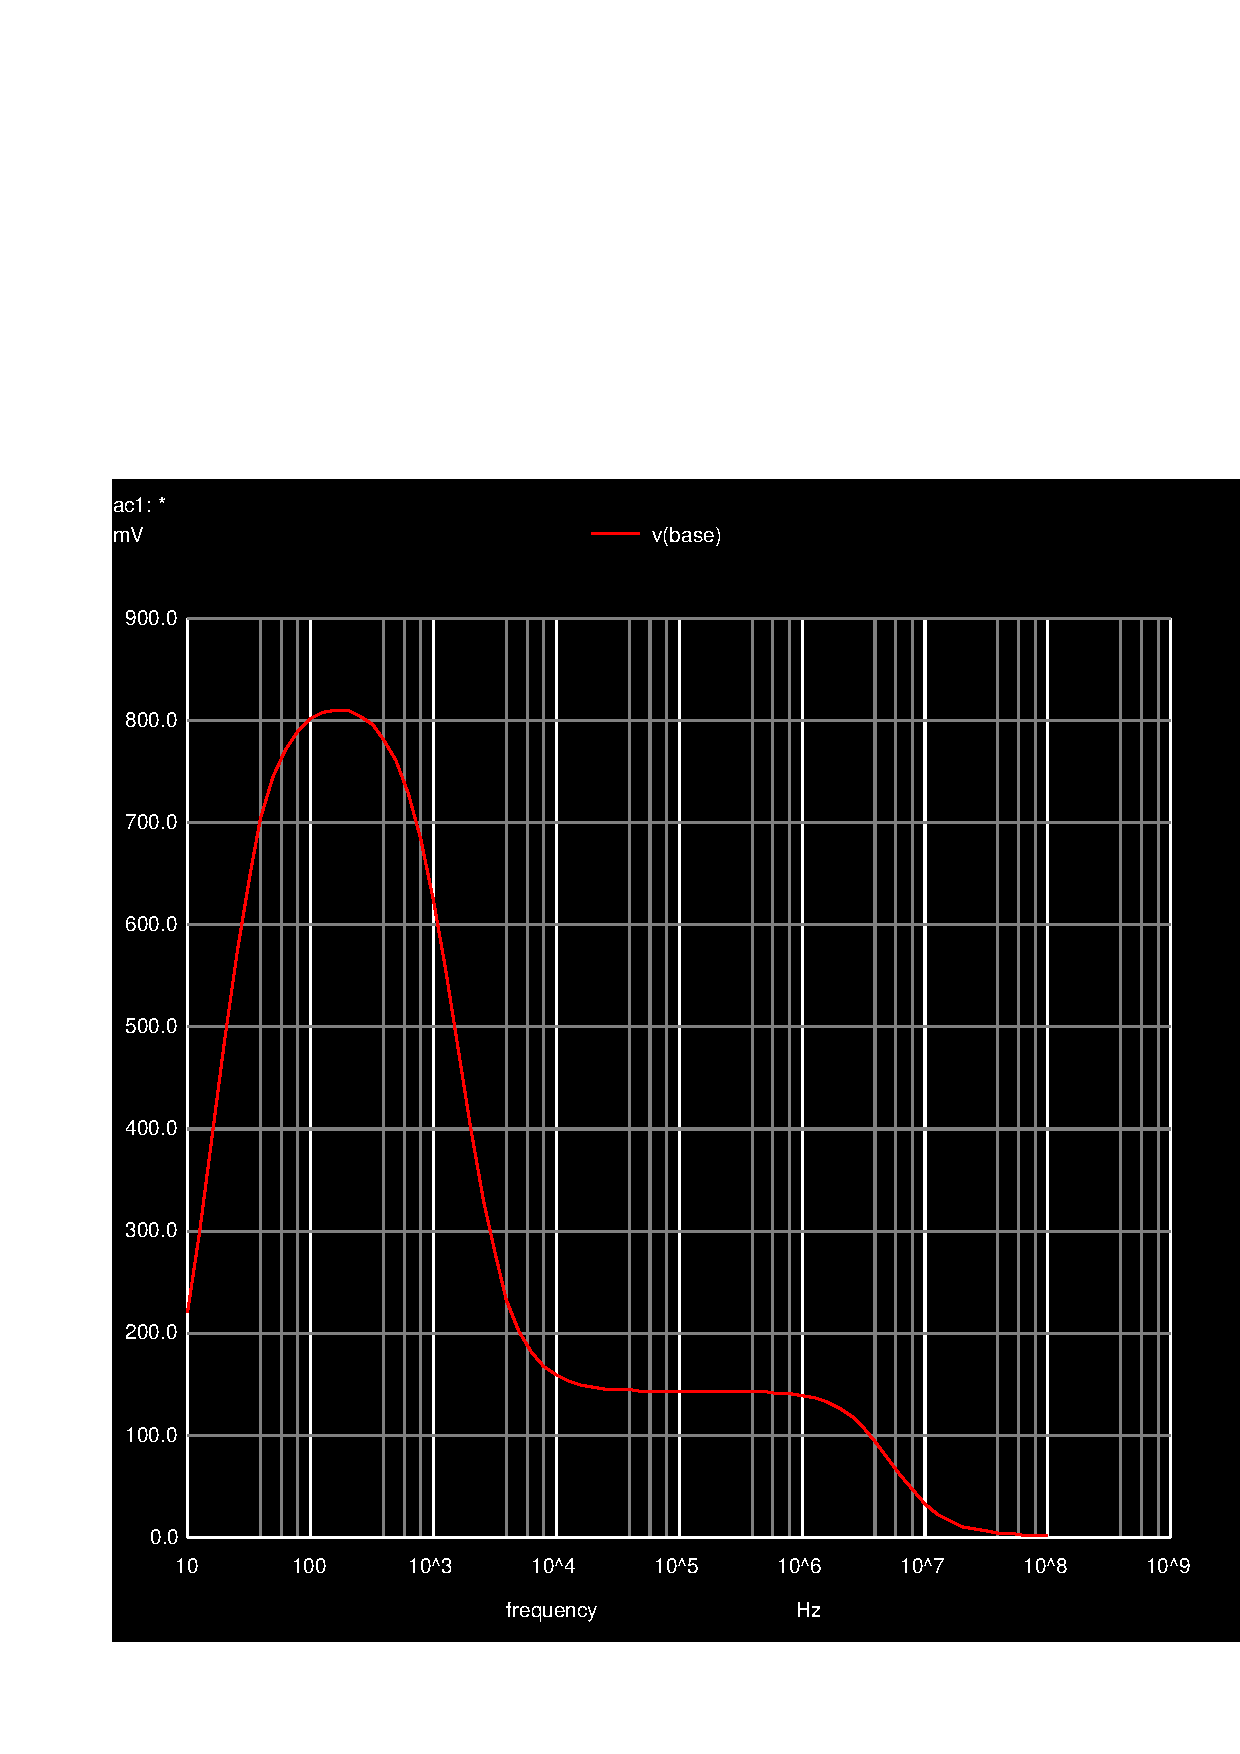
\includegraphics[width=0.8\columnwidth]{../sim/acp.pdf}
      \caption{Phase in degrees from ngspice}
      \label{fig:trans6}
    \endminipage\hfill
    \minipage{0.45\textwidth}
      \includegraphics[width=\linewidth]{T_angle.png} %../sim/
      \caption{Phase in degrees from matlab}
    \endminipage\hfill
\end{figure}
